\documentclass[UTF8]{mcmthesis}
\newtheorem{theorem}{Theorem}
\newtheorem{definition}[theorem]{Definition}
\newtheorem{corollary}{Corollary}[theorem]
\newtheorem{lemma}[theorem]{Lemma}
    % \usepackage{ctex}           % 暂时需要中文时添加, 最后注释掉即可
    \mcmsetup {
        tcn = 2416236, problem = C,    %% tcn is team control number
        titleinsummary = true,             %% title appears on summary sheet
    }

    % 调整 \item 的间距 
    \usepackage{paralist}
        \let\itemize\compactitem
        \let\enditemize\endcompactitem
        \let\enumerate\compactenum
        \let\endenumerate\endcompactenum
        \let\description\compactdesc
        \let\enddescriprion\endcompactdesc
    % 调整公式和正文的间距 (公式和正文更紧凑)
    \makeatletter
    \renewcommand\normalsize {
        % \@setfontsize\normalsize\@xpt\@xiipt
        \abovedisplayskip 5\p@ \@plus2\p@ \@minus5\p@
        \abovedisplayshortskip \z@ \@plus3\p@
        \belowdisplayshortskip 5\p@ \@plus3\p@ \@minus3\p@
        \belowdisplayskip \abovedisplayskip
        \let\@listi\@listI
    }
    \makeatother

    % \renewcommand{\baselinestretch}{1.2}      % 行间距
    \setlength{\parskip}{0.5em}                 % 段间距

    \usepackage{tikz}
        \usetikzlibrary{arrows} % 按需要添加扩展

    % 一般默认字体就好
    % \usepackage{mathptmx}     %% 数学公式罗马字体,对公式和正文都起作用
    % \usepackage{txfonts}      %% 数学公式罗马字体,对公式和正文都起作用
    % \usepackage{mathpazo}     %% COMAP 官方版物字体,对公式和正文都起作用
    % 一些重命名 ↓
    % \providecommand{\diff}{\mathop{}\!\mathrm{d}} %% 微分符号,正体 d
    % \providecommand{\me}{\mathrm{e}}              %% 无理数,正体 e
    % \providecommand{\mi}{\mathrm{i}}              %% 虚数单位,正体 i

    %% 设置目录节标题后加点
    \usepackage[titles]{tocloft}
    \renewcommand\cftsecdotsep{\cftdotsep}
    \renewcommand{\appendixpagename}{\Large\bfseries Appendices}

    %% 定制 Synopsis 页目录
    %% 根据需要把 Synopsis 改为 Memo or Handout 等等
    \fancypagestyle{Synopsis} {
        \fancyhf{}
        \lhead{\sffamily \team}
        \rhead{\sffamily Synopsis}
    }
    \title{\bfseries Do You Believe Momentum? A Mathematical Approach}  % 题目
  
\begin{document}
    \begin{summary}
    \begin{center}
        \textbf{Summary}
    \end{center}
	Our study delves into the intricate dynamics of match flow and the concept of momentum in tennis, using detailed point-by-point data from the Wimbledon 2023 Men's matches. Our primary focus was on developing a robust model to capture the flow of play and assess the impact of momentum in match outcomes. The study aimed to provide insights valuable in understanding and strategizing tennis matches. 
	
	\paragraph{Model Development and Visualization:}
	We developed a sophisticated model factoring in various match dynamics, including the advantage of serving, ace balls etc. The model effectively identified performance levels of players at different match stages. Visualization tools were employed to depict the flow of play.
	
	\paragraph{Assessment of Momentum:}
	Our analysis challenges the skepticism around momentum in tennis. We observed non-random patterns of play, contradicting the hypothesis that swings in a match are purely stochastic. The model indicated that momentum does have a tangible impact on match outcomes. 
	
	\paragraph{Predictive Analysis of Match Swings:}
	The model predicted shifts in the flow of play with over $60\%$ accuracy, identifying key indicators. This predictive capability provides a strategic tool for players and coaches in anticipating and adapting to match dynamics.
	
	\paragraph{Application and Testing on Other Matches:}
	When applied to other matches, the model demonstrated a high predictive accuracy, indicating its robustness. Some limitations were noted in matches with atypical play styles, suggesting areas for future enhancement.
	
	\paragraph{Generalizability and Cross-Sport Application:}
	We proposed a model that may apply to other matches as well. Insights from this study could extend to other sports with similar momentum dynamics, like table tennis.
	
	\paragraph{Conclusion and Recommendations for Coaches:}
	The study underscores the significance of momentum in tennis and other sports. We made a memo to coaches.

        %\vspace{2em}
        \noindent\textbf{Key Words: } Tennis Sport; Momentum; Neutral Network
\end{summary}

    \maketitle
    
    \newpage
    
    \tableofcontents
    
    \newpage
    \setlength{\parindent}{2em}
    \setcounter{page}{1}
    \section{Introduction}
    \subsection{Background Information}
    The 2023 Wimbledon Championships marked a significant event in the world of tennis, particularly in the Gentlemen's Singles category. One of the most notable matches was the final between the young Spanish sensation, 20-year-old Carlos Alcaraz, and the seasoned champion, 36-year-old Novak Djokovic. In a surprising turn of events, Alcaraz defeated Djokovic, ending the latter's impressive winning streak at Wimbledon since 2013. This match stood out not just for its outcome but also for its dramatic shifts in momentum, a concept often discussed in sports but hard to quantify. Throughout the match, both players exhibited periods of dominance, with the advantage oscillating between them in an unpredictable manner. This intriguing match, along with other games from the tournament, provides a rich dataset to explore the elusive concept of momentum in tennis and its impact on match outcomes.
	
	Momentum in sports has been studied by many scholars in various fields. Some aim to quantify momentum from a statisitical point of view, while others try to explain it from a sports psychological point of view. All fields are equally valid. However, our team will build a mathematical model to explain and answer the following questions:
	
	\begin{itemize}
		\item Create a model to capture the flow of play in tennis matches, identifying the player performing better at any given time and the extent of their advantage.
		\item Provide a visualization based on our model to depict the match flow.
		\item Use our model to evaluate the claim: "swings in a tennis match are random, as opposed to being influenced by momentum."
		\item Develop a model that predicts when the flow of play is about to change. Identify factors that might be related to these shifts.
		\item Test our model on other matches to evaluate its effectiveness and generalizability.
	\end{itemize}

	\subsection{Some Info on Tennis Scoring}
	\paragraph{Game}
	\begin{itemize}
		\item Each point won counts as one. 
		\item The first to score 4 points wins the game.
		\item At 3 points each, the score is 'Deuce.' From Deuce, a player must win by two points to win the game. 
		\item In international tennis, the scores of 0, 1, 2, and 3 points are represented by the English words Love, 15, 30, and 40, respectively.
	\end{itemize}
		
	\paragraph{Set}
	\begin{itemize}
		\item The first player to win 6 games wins the set.
		\item If both players win 5 games each, the set is won by the first player to lead by two games.
	\end{itemize}
		
	\paragraph{Tie-break Scoring}
	When the game score in a set reaches 6-all, one of the following tie-break methods is used:
	\begin{itemize}
		\item Long set: One player must lead by two games to win the set.
		\item Tie-break (or 'short set'): Except in the final set (unless otherwise specified), the following rules apply:
		\begin{itemize}
			\item The first player to score 7 points wins the game and the set (at 6-all, a player must win by two points).
			\item The first server serves the first point; thereafter, players alternate serving two consecutive points.
			\item The first point is served from the right court, the second from the left, and the third from the right.
			\item Players change ends after every six points and at the end of the tie-break.
		\end{itemize}
	\end{itemize}
		
	\paragraph{Best of Five Sets Format}
	The match is won by the player who first wins three out of five sets.

   \section{Who Has A Bigger Momentum? A Visualisation Approach}
	Before we begins any real development of our model, we need to visualise. Visualisation provides a clear and graphical approach. But, we need to state our definition for "momentum". In one of the academic papers we found, the authors \cite{chen-2020} identified momentum as:
	\begin{definition}[Momentum by Chen et al.]
		Score difference in a given period of time.
	\end{definition}
	\paragraph{Data Preprocessing}
	First we need to process some data in the csv file.
	\begin{itemize}
		\item Convert "match\_id" into unique sequential numbering
		\item Convert all time to seconds
		\item Standardise all scoring into points(e.g. 1,2,3). Reason being nonuniform scoring could affect calculation
	\end{itemize}
	
	Now, based on our definition of momentum, we have generated the following graphs. Original data are \color{gray} grey dots \color{black}, and \color{blue}blue trend-line \color{black}is drawn based on original data.
	
		
	\begin{figure}[H]
		\centering
		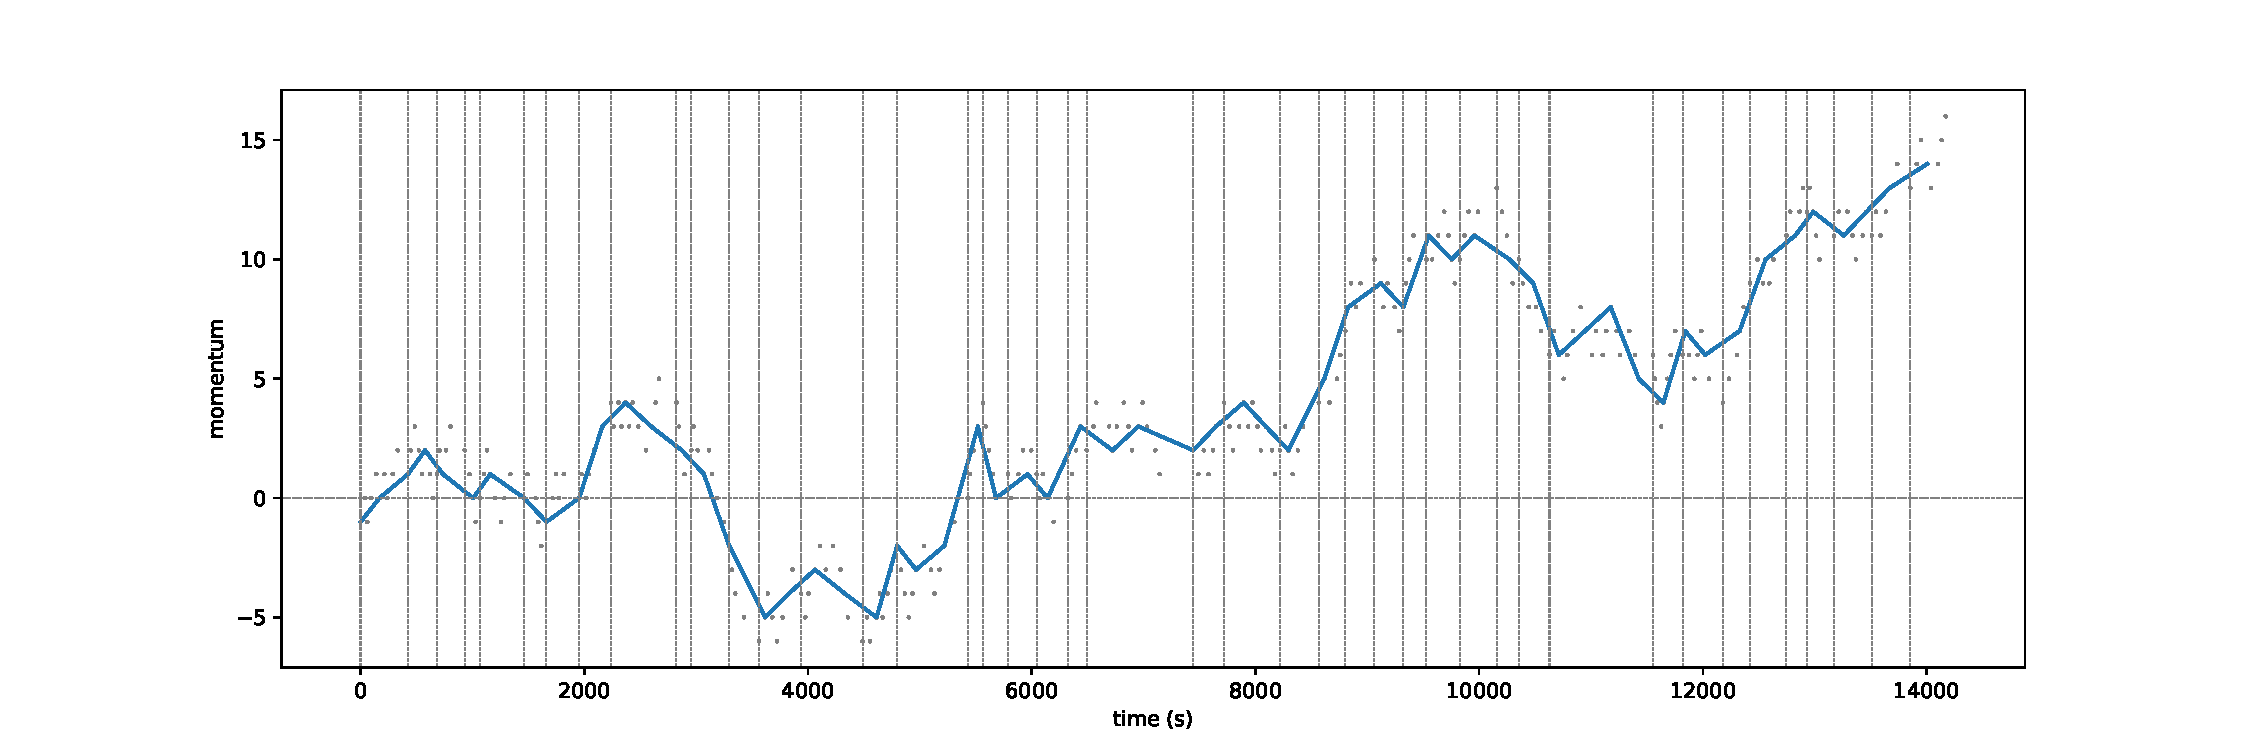
\includegraphics[width=1.0\linewidth]{figs/fig0_0.pdf}
		\caption{Global/Cumulative momentum(score difference) graph versus time, 1st match. Dotted lines separate each game. }
		\label{fig:fig0_0}
	\end{figure}	
	
	\begin{figure}[H]
		\centering
		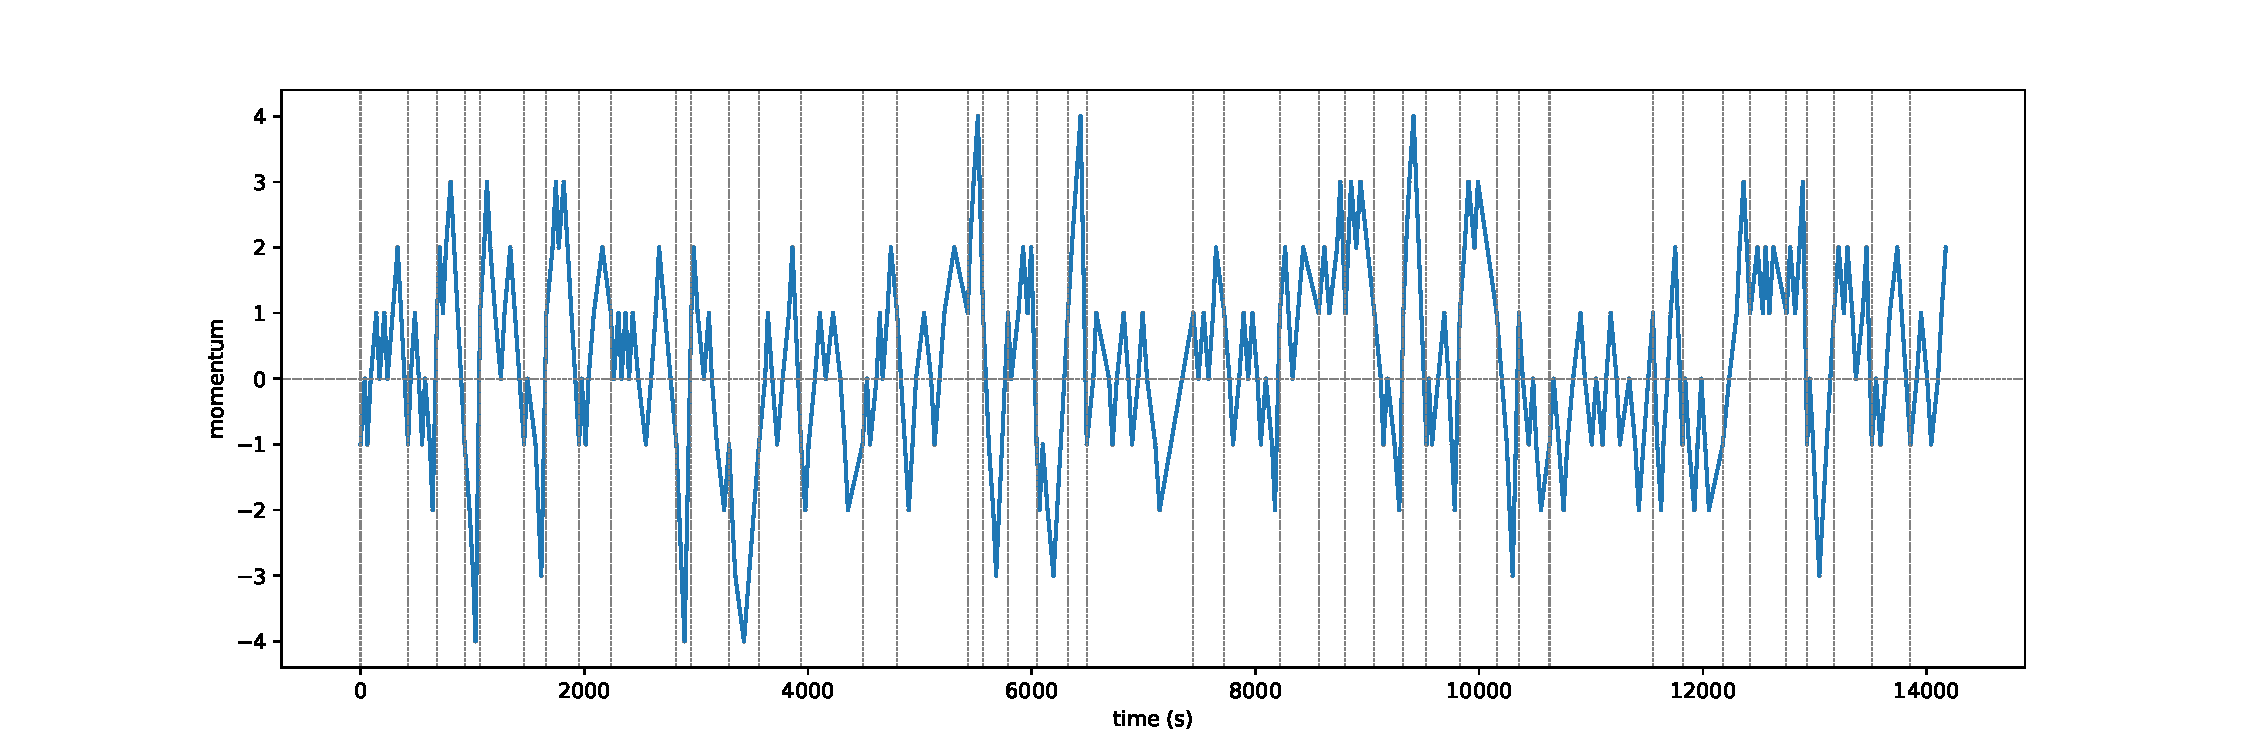
\includegraphics[width=1.0\linewidth]{figs/fig1_0.pdf}
		\caption{Momentum(score difference) of each game versus time, 1st match. Dotted lines separate each game.}
		\label{fig:fig10}
	\end{figure}
	
	
	We want a model that accounts for more than just score difference. We made 2 considerable additions to the definition of "momentum". 
	\begin{itemize}
		\item Added in "server advantage". Numerous papers have stated that server advantage is an important psychological effect to increase the probability of scoring\cite{Klaassen_1999} \cite{MacPhee_Pollard_2004}, though it alone does not determine the competition outcome. \textbf{We model the effect by adding a "server scoring probability" to whomever is serving.}
		\item Added in "ace". Ace means a server wins a point by serving. This significantly boosts the server's morale. 
	\end{itemize} 
	A modified visualisation shows:
	
	%
	%insert graphs here
	%
	\begin{figure}[H]
		\centering
		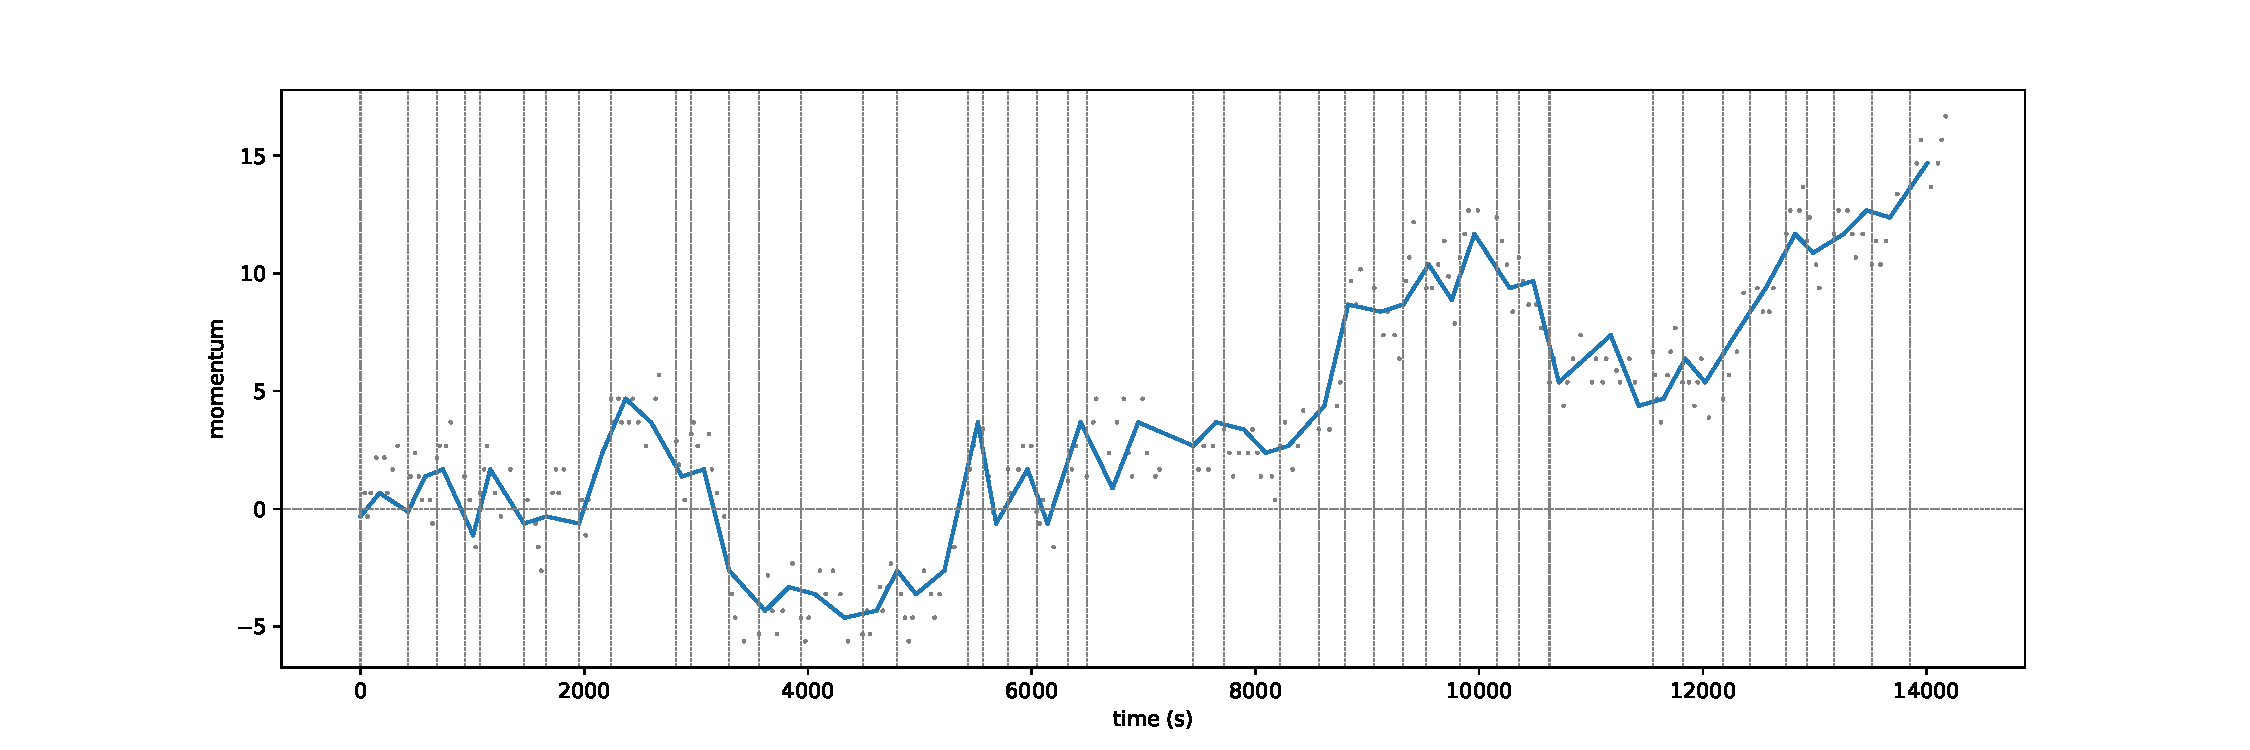
\includegraphics[width=1.0\linewidth]{figs/fig2_0.pdf}
		\caption{Modified global/cumulative momentum(score difference) graph versus time, 1st match. Dotted lines seperates each game.}
		\label{fig:fig2_0}
	\end{figure}
	
	\begin{figure}[H]
		\centering
		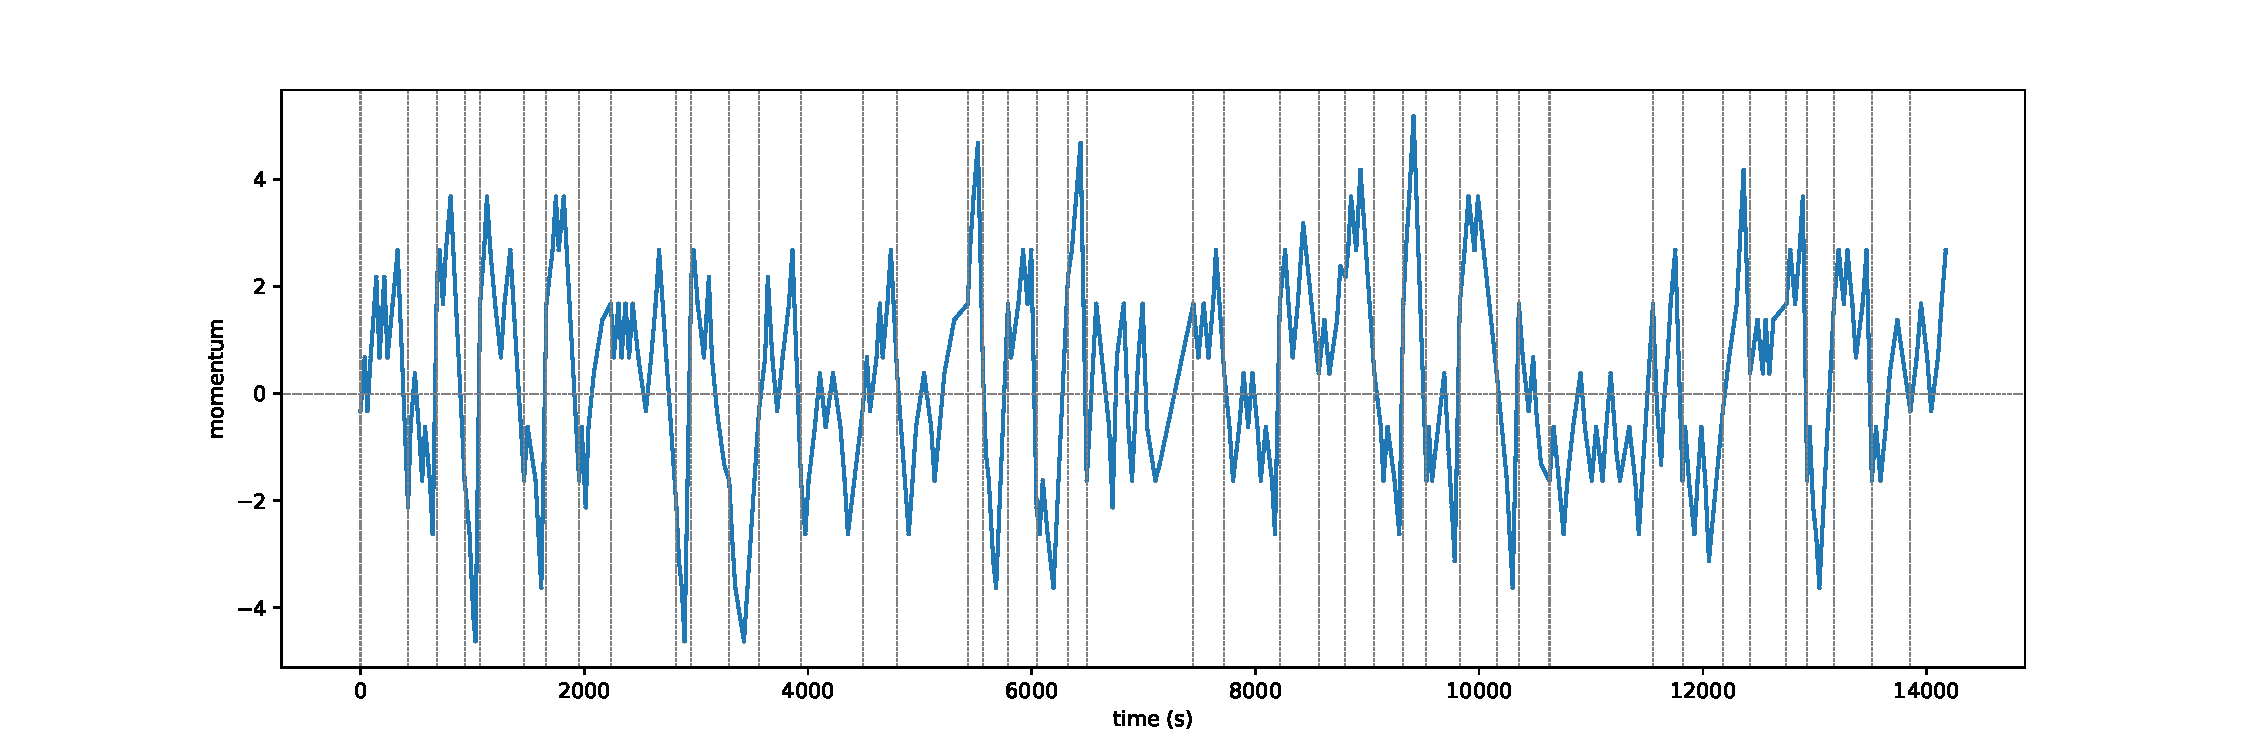
\includegraphics[width=1.0\linewidth]{figs/fig3_0.pdf}
		\caption{Modified momentum(score difference) of each game versus time, 1st match. Dotted lines sepaates each game.}
		\label{fig:fig30}
	\end{figure}
	
	\section{Do Swings Happen Randomly?}
	The study of momentum in sports generated great interests among scholars, sports coaches and athletes. The debate is still ongoing--some people do not believen in momentum\cite{Hale_2021}, just like our dear tennis coach.
	
	It was mentioned earlier that the trends of momentum rising and falling reflect performance. We can define the turning point of the rising and falling trends as the inflection point. In each game, by linearly fitting the overall performance of player 1 in the game with the number of balls scored, we can determine the slope that reflects the rising and falling trends. When the performance changes (i.e., when the sign of the slope changes), an inflection point occurs. To filter out the inflection points where the trend changes slowly, only |slope| above a certain threshold are considered as inflection points. These points are marked with red vertical lines on the graph.
	
	In this scenario, we aim to develop a mathematical model to identify turning points in a player's performance trend during a game. The turning points are defined as moments when the trend of performance changes from increasing to decreasing or vice versa, determined by the slope of a fitted line. 
	
	\begin{itemize}
		\item Data Representation
		\begin{itemize}
			\item Let \( t_i \) represent time in the game.
			\item Let \( y_i \) represent the player's score at each \( t_i \).
		\end{itemize}
		\item Linear Regression Model
		\begin{itemize}
			\item We use a simple linear regression model to fit the data points \((t_i, y_i)\).
			\item The linear model is given by \( y = mt + b \), where \( m \) is the slope and \( b \) is the y-intercept. The slope \( m \) indicates the trend of the player's performance. A positive slope implies an increasing trend, while a negative slope indicates a decreasing trend.
			\item To find the best-fit line, we minimize the sum of squared differences between the actual performance scores and the scores predicted by the linear model. The objective is to minimize the Mean Squared Error (MSE).
		\end{itemize}		
		\item Identifying Turning Points
		\begin{itemize}
			\item A turning point is identified when there is a change in the sign of the slope (from positive to negative or vice versa).
			\item Moreover, to filter out minor fluctuations, a threshold is set for the slope. Only when the absolute value of the slope changes and is greater than a specified threshold (in this case, 0.15) is a turning point acknowledged.
			\item Mathematically, if \( m_{prev} \) and \( m_{current} \) are the slopes of two consecutive segments and \( |m_{current}| > 0.15 \), a turning point is identified when \( \text{sign}(m_{prev}) \neq \text{sign}(m_{current}) \).
		\end{itemize}
	\end{itemize}
	
		We plotted turning points in momentum graphs. Original data are \color{gray} grey dots \color{black}, and \color{blue}blue trendline \color{black}is drawn based on original data. \color{red} Red lines \color{black} are turning points calculated based on original data. As figures below shows:
	
	\begin{figure}[H]
		\centering
		
		% Top subplot
		\begin{subfigure}[b]{\textwidth}
			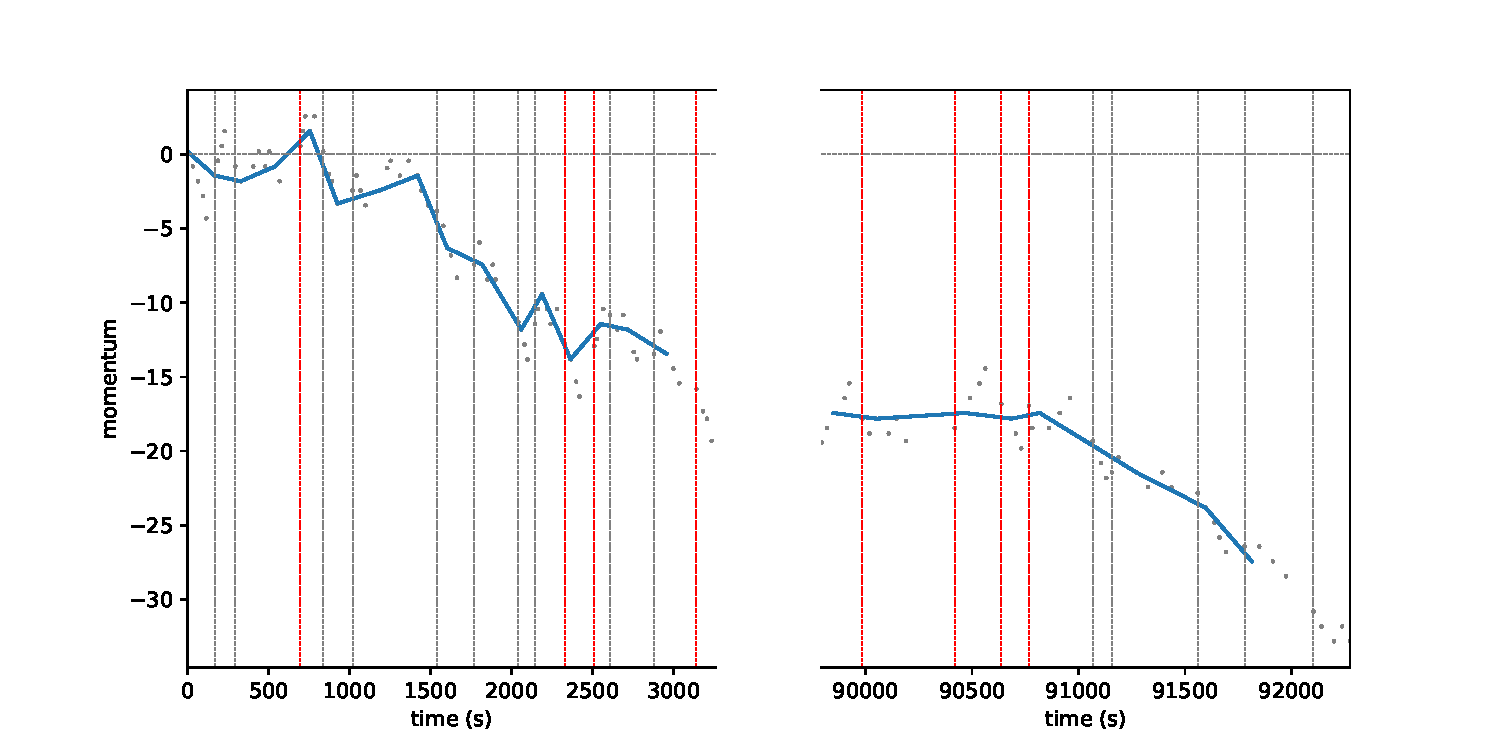
\includegraphics[width=1\linewidth]{figs/fig4_2.pdf}
			\caption{Modified global/cumulative momentum(score difference) graph versus time.}
			\label{fig:topfig4_2}
		\end{subfigure}
		
		% Add some space between the figures (optional)
		\vspace{1cm}
		
		% Bottom subplot
		\begin{subfigure}[b]{1.0\textwidth}
			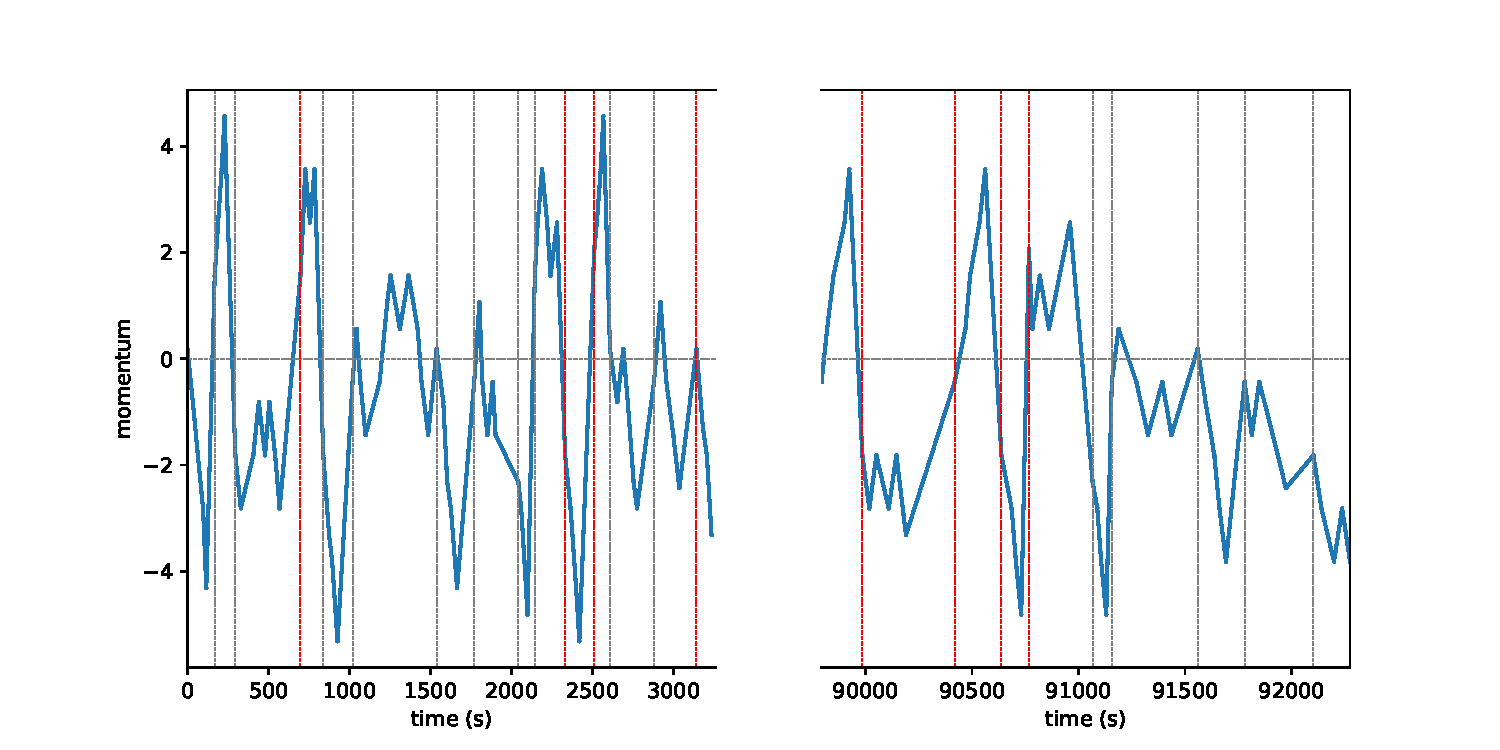
\includegraphics[width=1\linewidth]{figs/fig5_2.pdf}
			\caption{Modified momentum(score difference) of each game versus time.}
			\label{fig:bottomfig5_2}
		\end{subfigure}
		
		\caption{3rd match. Dotted lines seperates each game. Dotted red lines indicate swings}
		\label{fig:both_figures2}
	\end{figure}
	
	\begin{figure}[H]
		\centering
		
		% Top subplot
		\begin{subfigure}[b]{\textwidth}
			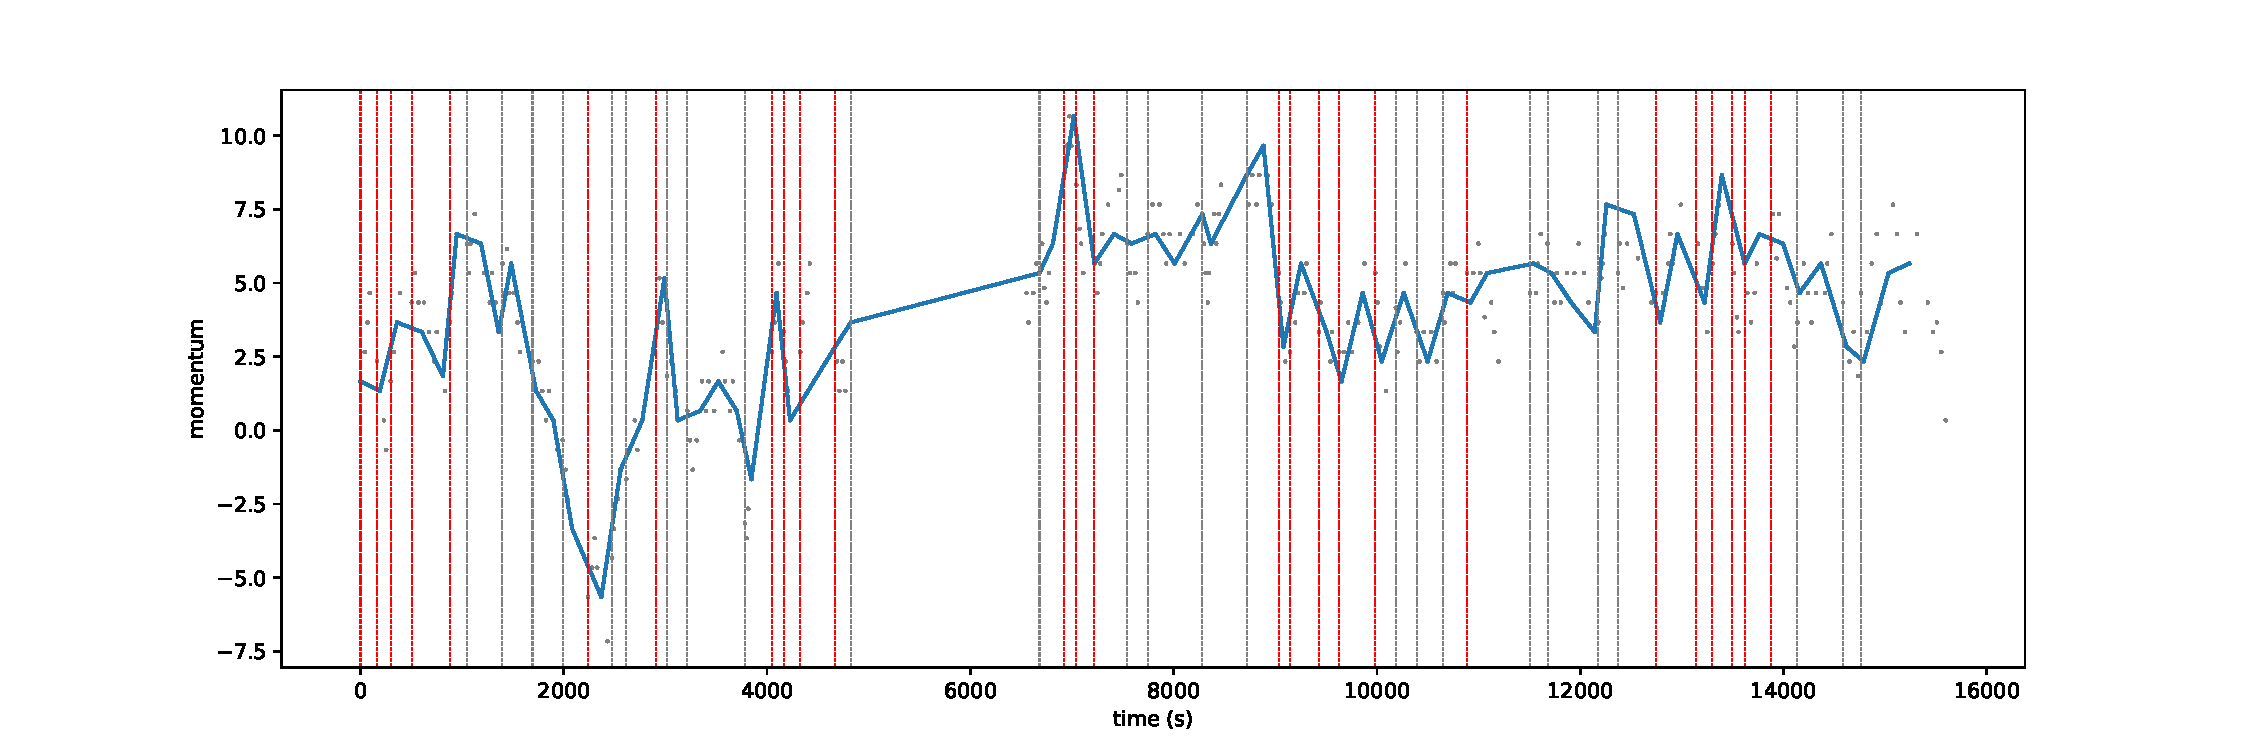
\includegraphics[width=1\linewidth]{figs/fig4_3.pdf}
			\caption{Modified global/cumulative momentum(score difference) graph versus time.}
			\label{fig:topfig4_3}
		\end{subfigure}
		
		% Add some space between the figures (optional)
		\vspace{1cm}
		
		% Bottom subplot
		\begin{subfigure}[b]{1.0\textwidth}
			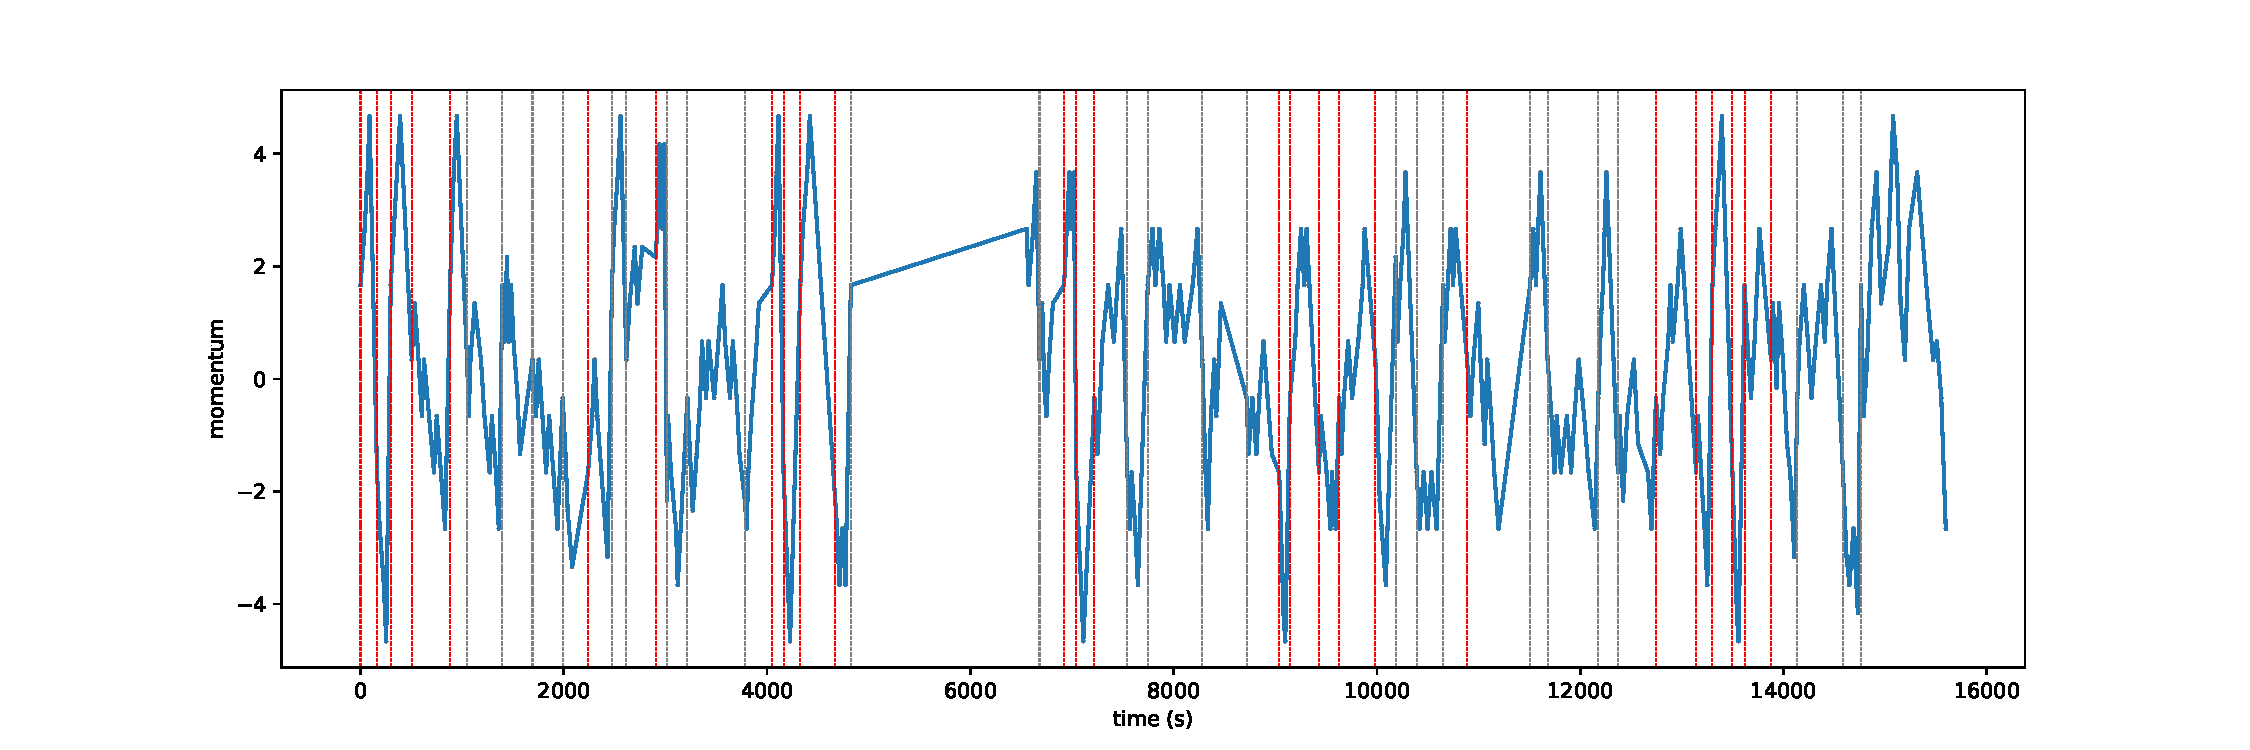
\includegraphics[width=1\linewidth]{figs/fig5_3.pdf}
			\caption{Modified momentum(score difference) of each game versus time.}
			\label{fig:bottomfig5_3}
		\end{subfigure}
		
		\caption{4th match. Dotted lines sepaates each game. Dotted red lines indicate swings}
		\label{fig:both_figures3}
	\end{figure}
	
	Now we have identified all turning points that are actually swings, we need to test for their randomness. We have imposed certain conditions on turning points and the randomness test is as follows:
		
	Let's denote:
	\begin{enumerate}
		\item \( N \) as the total number of games.
		\item \( n_1 \) as the number of games with turning points.
		\item \( n_2 \) as the number of games without turning points.
		\item \( N = n_1 + n_2 \).
		\item \( R \) as the total number of runs (a run is a sequence of consecutive games either all with turning points or all without turning points).
	\end{enumerate}
		
	The expected number of runs (\( E(R) \)) and the variance of the number of runs (\( Var(R) \)) are given by:
	\begin{enumerate}
		\item \[ E(R) = \frac{2n_1n_2}{N} + 1 \]
		\item \[ Var(R) = \frac{2n_1n_2(2n_1n_2 - N)}{N^2(N - 1)} \]
	\end{enumerate}
	
	The test statistic (\( Z \)) is then calculated as:
	\[ Z = \frac{R - E(R)}{\sqrt{Var(R)}} \]
	
	While P-value is given by:
	\[ \text{p-value} = 2P(Z > |z|) \]
	Interpretation	
	\begin{itemize}
		\item If the value of \( Z \) is significantly high or low, it indicates that the turning points are not randomly distributed, suggesting a pattern or trend in the player's performance changes.
		\item A low p-value (< 0.05) means reject the null hypothesis.
	\end{itemize}
	
    We calculated the p-value and \( Z \) of all matches. We found that most of the p-values are super low, such as 9.18e-5 and 6.82e-4.(You can find it in appendices) They are much less than 0.05. So we can conclude that we reject the null hypothesis. Or we can conclude that the data is not random. Also, the significantly high \( Z \) value, such as -3.89 and -3.40, shows the same conclusion.

	\paragraph{Results}
	We have obtained very low p-values and high Z-score, which suggests that swings are not random.
	
	\section{How To Predict Swings?}
	As soon as we have tested the non-randomness of swings, a new question immediately surfaces: can we predict the flow of play? This is very important to sports coaches as it can be used for post-match analysis. Fear not! We have developed a model using deep learning.
	
	But the first step might be the most important step. In order to predict swings, or turning points in a match, we shall first consider the most influential parameters that can have impact on a player’s performance, which can be deduced by the information from the preceding few points. Such parameters are called \textbf{features}.
	
	\subsection{Feature Engineering}
	In our data analysis, the critical parameters that have great impact on dependent variable, or anticipated value shall be regarded as features. Since we have too much data, we shall introduce the method of machine learning. We must feed ML algorithms data in the form of features, to aid in efficient predictions. In our case, predict the performance of each player and if a “swing of momentum” is going to occur.
	
	However, the validity and feasibility of machine learning remarkably depends on the selection and processing of features, due to the different importance of parameters. We shall process the data in a way that generates features that has the greatest correlation on the output. Such step is known as feature engineering, which is the most time-spending but the most critical step in machine learning.
	
	

	\begin{itemize}
		\item Dependent Variable: Whether a player scores a point (binary 1 or 0), essentially predicting the probability of a player scoring in the next rally.
		\item Independent Variables: Data from all past rallies in the match.
	\begin{table}[!ht]
    \centering
    \begin{tabular}{|l|l|}
    \hline
        global features & explanation  \\ \hline
        match score & how many sets the players have won in the present match  \\ \hline
        set score & how many games the players have won in the present set  \\ \hline
        game score & how many points the players have won in the present game  \\ \hline
        elapsed time & how much time has elapsed during the match  \\ \hline
        total point & how much points the players have already played in the match  \\ \hline
    \end{tabular}
    \label{global features}
    \end{table}
    
    \begin{table}[!ht]
    \centering
    \begin{tabular}{|l|l|}
    \hline
        serve features & explanation  \\ \hline
        server & who is going to serve at the present point.  \\ \hline
        aces & nonreturnable or untouchable serves.  \\ \hline
        serve number  & the first time or the second time that the server served successfully  \\ \hline
        serve width & the distance between the receiver and the serve  \\ \hline
        serve depth & the distance between the serve's ground-touching point and the line  \\ \hline
        serve speed & the speed of the serve  \\ \hline
        double faults & occasions in which the server fails to serve successfully for two times  \\ \hline
        return depth & whether the return of the serve is deep  \\ \hline
    \end{tabular}
    \label{global features}
\end{table}
    
    \begin{table}[!ht]
    \centering
    \begin{tabular}{|l|l|}
    \hline
        rally features & explanation  \\ \hline
        winner & untouchable shot due to large power or tricky ball-hitting direction  \\ \hline
        winner type & forehand or backhand winner  \\ \hline
        net point & a point in which a player goes to the net  \\ \hline
        net point winner & a point in which a player goes to the net and wins  \\ \hline
        unforced error & someone losing a point not due to the pressure of the opponent  \\ \hline
        rally count & total hits of balls during a point  \\ \hline
        running distance & running distance of a player during a point  \\ \hline
    \end{tabular}
    \label{global features}
\end{table}
        
        \begin{table}[!ht]
    \centering
    \begin{tabular}{|l|l|}
    \hline
        critical point features & explanation  \\ \hline
        break point & a point at which the receiver has the game point  \\ \hline
        break point missed & a point at which the receiver misses the game point  \\ \hline
        break point won & a point at which the receiver wins the game point  \\ \hline
    \end{tabular}
\end{table}%% 表格部分结束
	\end{itemize}
	\subsubsection{The Summary of Features}
	After having briefly listed some features that describe a tennis match, we want to summarize the features and, because there are too many of them, and we should also rewrite the features in a manner that is suitable for machine learning.\\
	Among the features listed above, we found out there are few that play a more role more crucial than others:\\
	\begin{itemize}
	\item \textbf{The Server:}
	 the server has way more advantage than the receiver in his game of serving: In professional games, the speed of the serve can reach up to more than 120 mph. On May 9, 2012, in Busan, South Korea, Australian player Sam Groth hit the world’s fastest serve at 163.7 mph (263.4 kph)$^{[a]}$ , around the taking off speed of commercial airliners(160-180mph)$^{[b]}$ . Such powerful serves are generally indefensible. The serve is the only thing in tennis match that a player can handle in his hands completely, that’s why players practice hard to serve as powerfully as possible.
	 \item \textbf{First/Second Serve:}
	 An athlete has two chances to serve in each point, their first attempt is called the first serve, while their second attempt is called the second serve. Generally, the first serve is more powerful than the second serve, since the player knows that he still holds a chance even if he fails the first serve. based on data gathered from over 100 ATP Tour players, the average speed of first and second serves are as follows$^{[c]}$: 
\\Average First Serve Speed: 115.79 mph (186.35 km/h)
\\Average Second Serve Speed: 94.44 mph (151.98 km/h)
    \item \textbf{Aces:}
     by definition, An ace is a serve that successfully lands in the service box and does not touch the receiving player’s racquet$^{[c]}$.  Typically, a player will hit an ace on their first serve, where the speed of the ball tends to be greater than a second serve. Actually, an ace is a winner that guarantees the server for obtaining a point.
     \item \textbf{Double Fault:}
      The server has two attempts to make their serve. If they miss their first attempt to hit their serve into the correct service box, it’s a fault. The second miss of their serve results in a double fault causing the server to lose the point$^{[d]}$. 
       \item \textbf{Winner:}
       By definition, if a player hits a shot within bounds of their opponent’s side of the court that they can’t reach, the point is called a winner$^{[e]}$.
       \item \textbf{Net Point:} 
       if during a point a player goes to the net, attempting to hit the ball before falling on the ground, the point is called a net point.
       \item \textbf{Unforced error: } 
       Unforced errors are those types of mistakes that are supposedly not forced by good shots of an opponent. Generally, if you see a player surprisingly missed a shot which can be brought as a winner, that is surely an unforced error.$^{[f]}$
       \\As is seen by the introduction, these are several relatively more important features in tennis games.
	\end{itemize}
	\subsubsection{ The Specification of Features}
	By specifying features quantitatively, we turn abstract concepts into concrete data. But how are we able to do that? This is also an important procedure in feature engineering during which we analyze the given data and calculate the features that we want.
    Based on our observation, we have theorized a few statements:\\
    \textbf{1. Compared to global features, local features are relatively better indicators for A single player’s performance.}\\\\
\textbf{2. Local features can be deduced by the information contained by several points preceding the target point, which is the point that we want to predict (who’s going to win the point or a swing of momentum is coming).}\\\\
\textbf{3. Such local features can be regarded as the cumulative advantage ( or disadvantage ) of one player against the other in the last few(n) points.}\\
\begin{table}[!ht]
    \centering
    \begin{tabular}{|l|l|}
    \hline
        final features & explanation  \\ \hline
        serve\_index & $    \begin{cases}  1 & \text{if server} = \text{player1} \\-1 & \text{if server} = \text{player2}  \end{cases}$ \\ \hline
        games\_in\_lead & $ \text{set\_score}(\text{player1}) - \text{set\_score}(\text{player2})$ \\ \hline
        last\_point\_index & $ \begin{cases} 1 & \text{if player1 has won the last point} \\-1 & \text{if player2 has won the last point}  \end{cases}$ \\ \hline
        ace\_advantage & $  \sum_{j=i-n}^{i-1} N_{\text{player1}}^{\text{aces}} - \sum_{j=i-n}^{i-1} N_{\text{player2}}^{\text{aces}}$ \\ \hline
        winner\_advantage & $ \sum_{j=i-n}^{i-1} N_{\text{player1}}^{\text{winners}} - \sum_{j=i-n}^{i-1} N_{\text{player2}}^{\text{winners}}$ \\ \hline
        double\_fault\_disadvantage & $  \sum_{j=i-n}^{i-1} N_{\text{player1}}^{\text{double\_faults}} - \sum_{j=i-n}^{i-1} N_{\text{player2}}^{\text{double\_faults}}$ \\ \hline
        unforced\_error\_disadvantage & $ \sum_{j=i-n}^{i-1} N_{\text{player1}}^{\text{unforced\_errors}} - \sum_{j=i-n}^{i-1} N_{\text{player2}}^{\text{unforced\_errors}}$ \\ \hline
        net\_winner\_advantage & $ \sum_{j=i-n}^{i-1} N_{\text{player1}}^{\text{net\_winners}} - \sum_{j=i-n}^{i-1} N_{\text{player2}}^{\text{net\_winners}}$ \\ \hline
        winning\_break\_point\_advantage & $ \sum_{j=i-n}^{i-1} N_{\text{player1}}^{\text{break\_points}} - \sum_{j=i-n}^{i-1} N_{\text{player2}}^{\text{break\_points}}$ \\ \hline
        running\_distance\_advantage & $ \sum_{j=i-n}^{i-1} N_{\text{player2}}^{\text{running\_distance}} - \sum_{j=i-n}^{i-1} N_{\text{player1}}^{\text{running\_distance}}$ \\ \hline
        first\_serve\_advantage & $ \sum_{j=i-n}^{i-1} N_{\text{player1}}^{\text{first\_serve}} - \sum_{j=i-n}^{i-1} N_{\text{player2}}^{\text{first\_serve}}$
 \\ \hline
    \end{tabular}
\end{table}
	\subsubsection{Normalization and Standardization of the Features}
	After obtaining a series of features, the last step we are going to is to standardize, or to normalize the vectors, so that the scale of different features will not influence the process of machine learning.\\
	The most commonly used way of normalization is Min-Max normalization, in which we do a transformation to a feature so that every value fall inside the range between 0 and 1, and the formula is as shown:\\
	\begin{equation*}
	    x^{'}=\frac{x-x_{min}}{x_{max}-x_{min}}
	\end{equation*}
	There is another way of standardization, called the "z-score standardization." In z-score standardization, we do a transformation to a feature so that the average value of the feature is 0 and its standard deviation is 1:
	\begin{equation*}
	    x^{'}=\frac{x-\overline{x}}{\sigma}
	\end{equation*}
	The two different normalization are necessary and crucial for machine learning methods, such as KNN, which require the computation of distance. In our computation, we apply min-max normalization to our data.
	
	
	
	
	\subsection{Regression Model}
	After preparing data, we decided to use a 2-layer linear regression model to train the data. The neural network is a simple feedforward network with two linear layers and a ReLU activation function in between.
	
	\begin{itemize}
		\item Layers:
		\begin{itemize}
			\item First Linear Layer: This layer takes the input vector \( \mathbf{x} \in \mathbb{R}^{n} \) (where \( n \) is the number of features) and transforms it to a hidden vector \( \mathbf{h} \in \mathbb{R}^{m} \) (where \( m \) is the size of the hidden layer, 256 in our case). The transformation is defined as: 
			\[ \mathbf{h} = \mathbf{W}_1 \mathbf{x} + \mathbf{b}_1 \]
			where \( \mathbf{W}_1 \in \mathbb{R}^{m \times n} \) is the weight matrix and \( \mathbf{b}_1 \in \mathbb{R}^{m} \) is the bias vector of the first layer.
			\item ReLU Activation: The ReLU (Rectified Linear Unit) function is applied element-wise to the hidden vector \( \mathbf{h} \). It is defined as:
			\[ \text{ReLU}(h_i) = \max(0, h_i) \]
			for each element \( h_i \) of \( \mathbf{h} \).
			\item Second Linear Layer: This layer maps the hidden vector \( \mathbf{h} \) to the output \( y \in \mathbb{R} \). The transformation is:
			\[ y = \mathbf{W}_2 \mathbf{h} + b_2 \]
			where \( \mathbf{W}_2 \in \mathbb{R}^{1 \times m} \) is the weight matrix and \( b_2 \in \mathbb{R} \) is the bias of the second layer.
		\end{itemize}
		\item  Training:
		\begin{itemize}
			\item Loss Function: The model uses Mean Squared Error (MSE) as the loss function.
			\item Optimization: The Adam optimizer is used to minimize the loss function. Adam is an adaptive learning rate optimization algorithm that's considered effective for deep learning models.
		\end{itemize}
		\item Prediction: The final model takes an input vector \( \mathbf{x} \), processes it through the layers as described, and outputs a prediction \( y \).		
	\end{itemize}
	
	After 1000 epoches of training, our final result is $\text{Loss}=0.2189$, while $\text{MSE}=0.2287$. 
	
	\begin{figure}[H]
		\centering
		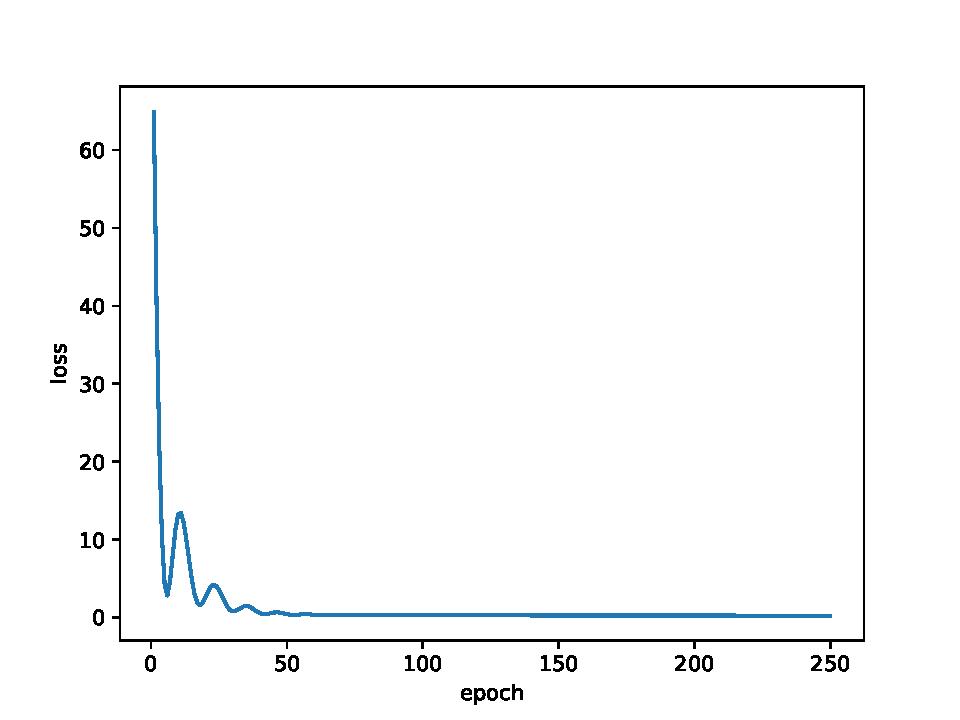
\includegraphics[width=1.0\linewidth]{figs/fig6.pdf}
		\caption{Loss versus epoch graph. X-axis is trimmed because loss converges to 0.22 from 250 epoches onwards.}
		\label{fig:fig6}
	\end{figure}
	
	
	Based on this model, we plotted a graph of \color{blue}{actual swings} \color{black} and \color{red}{predicted swings} \color{black}. The accuracy from our model stands around $70\%$
	
	
	\begin{figure}[H]
		\centering
		
		% Top subplot
		\begin{subfigure}[b]{\textwidth}
			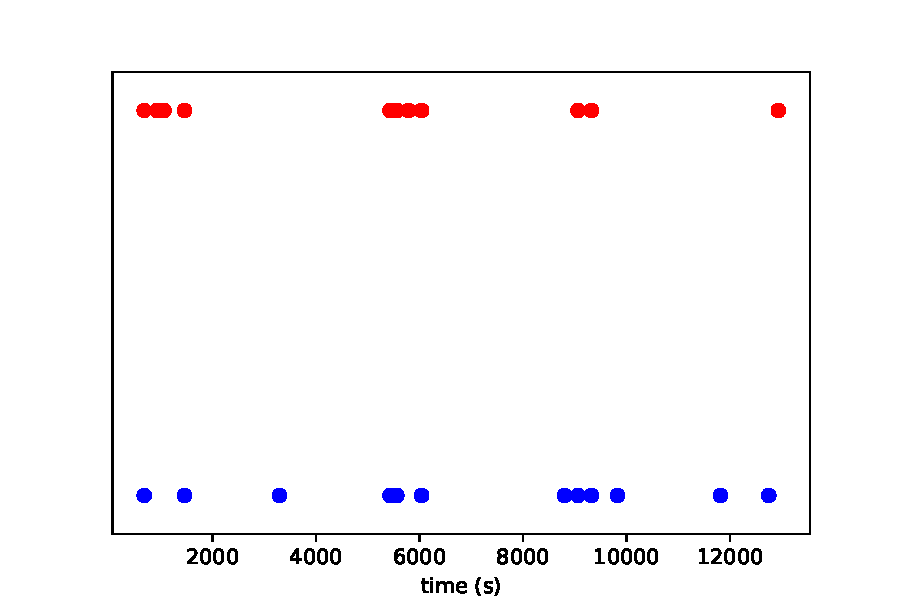
\includegraphics[width=1\linewidth]{figs/fig7_0.pdf}
			\caption{1st match}
			\label{fig:topfig7_0}
		\end{subfigure}
		
		% Add some space between the figures (optional)
		\vspace{1cm}
		
		% Bottom subplot
		\begin{subfigure}[b]{\textwidth}
			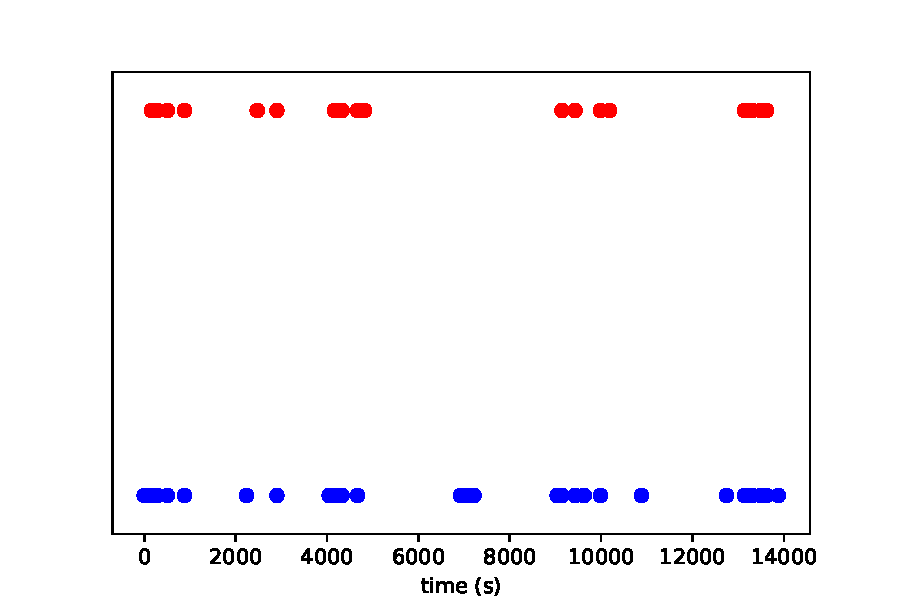
\includegraphics[width=1\linewidth]{figs/fig7_3.pdf}
			\caption{4th match}
			\label{fig:bottom}
		\end{subfigure}
		
		\caption{Predicted swings(red) versus actual swings(blue)}
		\label{fig:both_figures}
	\end{figure}
	
	
	
	\subsection{Classification Model}
	We have tested another deep learning model against our data. The text below outlines how our model works:
	
	\begin{itemize}
		\item Layers:
		\begin{itemize}
			\item Input Layer: Number of nodes equals the number of input features. Let's denote this number as \( n \).
			\item Hidden Layer: Consists of 256 nodes. This layer uses a ReLU (Rectified Linear Unit) activation function.
			\item Output Layer: 2 nodes, corresponding to the classification categories. This layer uses a Softmax activation function for probability distribution.
		\end{itemize}
		\item From Input to Hidden Layer:
		\begin{itemize}
			\item Let \( \mathbf{x} \in \mathbb{R}^{n} \) be the input vector of size \( n \).
			\item The weights connecting the input layer to the hidden layer can be represented as a matrix \( \mathbf{W_1} \in \mathbb{R}^{256 \times n} \).
			\item The bias for the hidden layer is a vector \( \mathbf{b_1} \in \mathbb{R}^{256 \times 1} \).
			\item The output of the hidden layer before activation, \( \mathbf{H} \), is given by  \( \mathbf{H} = \mathbf{W_1} \mathbf{x} + \mathbf{b_1} \), where \( \mathbf{H} \in \mathbb{R}^{256 \times 1} \).
			\item After applying ReLU, the output of the hidden layer becomes \( \mathbf{H'} = \max(0, \mathbf{H}) \), with \( \mathbf{H'} \in \mathbb{R}^{256 \times 1} \).
		\end{itemize}
		\item From Hidden to Output Layer:
		\begin{itemize}
			\item The weights from the hidden layer to the output layer can be represented as a matrix \( \mathbf{W_2} \in \mathbb{R}^{2 \times 256} \).
			\item The bias for the output layer is a vector \( \mathbf{b_2} \in \mathbb{R}^{2 \times 1} \).
			\item The final output before applying softmax, \( Y \), is given by \( Y = \mathbf{W_2} \mathbf{H'} + \mathbf{b_2} \).
			\item The Softmax function is applied to \( Y \) to get the probability distribution over the two classes. If \( Y = [y_1, y_2] \), the softmax function is defined as \( Y = \mathbf{W_2} \mathbf{H'} + \mathbf{b_2} \), where \( Y \in \mathbb{R}^{2 \times 1} \).
		\end{itemize}
		\item Loss Function:
		\begin{itemize}
			\item The model uses Cross-Entropy Loss, which is commonly used in classification tasks. For a single instance with true label \( c \) and predicted probabilities \( p_1, p_2 \), the cross-entropy loss is:
			 \[ \text{Loss} = -\sum_{i=1}^{2} \mathbf{1}(c = i) \log(p_i) \]
			where \( \mathbf{1}(c = i) \) is the indicator function, equal to 1 when \( c = i \) and 0 otherwise.
		\end{itemize}
		\item Optimization:
		\begin{itemize}
			\item Adam Optimizer: This is used for adjusting the weights \( \mathbf{W_1}, \mathbf{W_2} \) and biases \( \mathbf{b_1}, \mathbf{b_2} \) to minimize the loss function. Adam is an adaptive learning rate optimization algorithm that combines the advantages of two other extensions of stochastic gradient descent, namely AdaGrad and RMSProp.
		\end{itemize}
		\item Model Evaluation:
		\begin{itemize}
			\item After training, the model's performance is evaluated by its accuracy on the test dataset. For predicted labels \( \hat{y} \) and true labels \( y \), accuracy is defined as:
			\[ \text{Accuracy} = \frac{\text{Number of Correct Predictions}}{\text{Total Number of Predictions}} = \frac{\sum_{i=1}^{N} \mathbf{1}(\hat{y}_i = y_i)}{N} \]
			where \( N \) is the total number of predictions.
		\end{itemize}
	\end{itemize}
	
	After 300 epoches of training, we achieved an accuracy of $63.96\%$. The loss-epoch diagram is shown below:
		
	\begin{figure}[H]
		\centering
		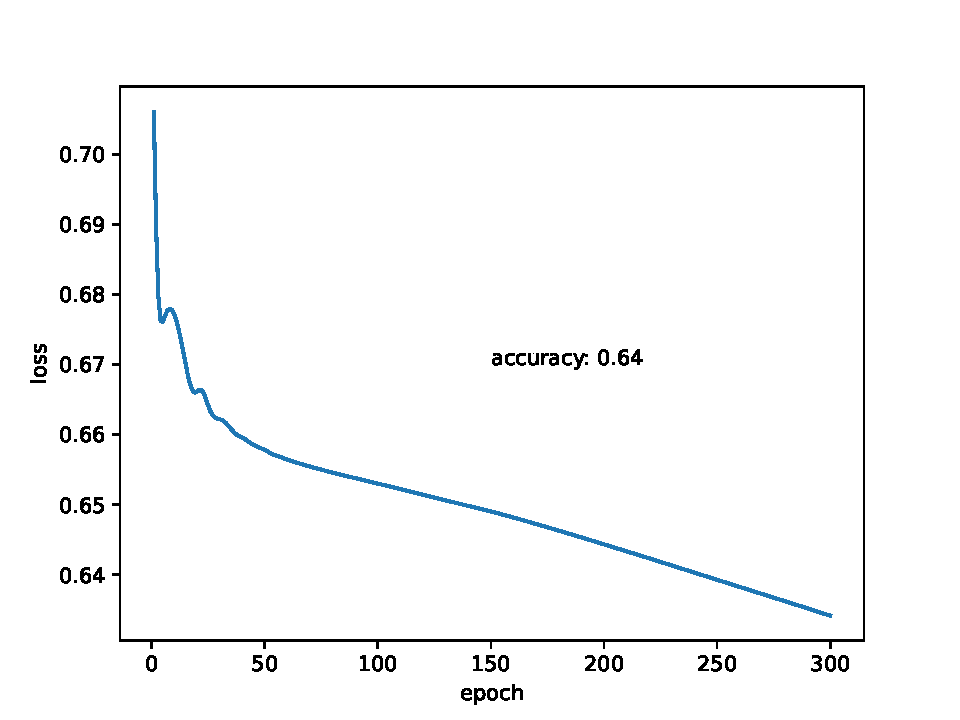
\includegraphics[width=1\linewidth]{figs/fig8.pdf}
		\caption{Loss versus epoch graph for classification model. Accuracy is around 0.64}
		\label{fig:fig8}
	\end{figure}
	
	One thing should be stressed: the classification model does not predict the swing (turning point). This model is used to predict whether the player will get the next point.
	
	The model in the above section developed a good method to predict the momentum turning points. Coaches who want to predict the turning points of the match can monitor the data and use it for calculation. By using the model above, coaches can predict the turning points of a specific match. We used our model to predict turning points in some matches. Figure \ref{fig:both_figures} shows the prediction of 1st match and 4th match. We can see that our model predicted most of the time intervals which include turning points. For every single turning point, the accuracy is approximately $70\%$. We also found that being the server has important influence on the distribution of turning points. And winning streak accumulation is also a major influencing factor.
            

    \section{Discussion on Our Model}
    
    \subsection{How a Player Prepare the Match?}
    Before the competition, athletes can collect information about their own and their opponent's data in advance. After filtering out features from these data, we can use our model to simulate possible scenarios during the competition. Prepare for key points in advance based on simulated data. In addition, during the competition, it is necessary to monitor relevant data in real time, and use our model to predict the momentum swings based on relevant data. These information can be used to one's advantage.
    
    
    
    \subsection{Further Discussion on Our Model}
    
    In terms of score prediction accuracy, our model still has certain flaws. We found that in addition to server advantage, ace balls, hitting speed, hitting time, etc., also have a great impact on scoring. In future models, we need to make better quantification in order to achieve better training results. In addition, factors such as the player's historical performance also need to be considered. Future models can achieve better prediction results by building player databases and training different models for different players.
    
    

    Another issue is the generality of our model. For tennis matches, our model has strong generality. The rules of tennis matches are basically the same, and the factors affecting scoring are relatively fixed, so we expect our model to achieve good results. For other ball sports, we need to consider the sources of momentum in these sports. For sports with similarities (such as similar advantages of serving, serving speed, etc.), we also expect our model to have good results. However, due to data and time constraints, we have not seriously analyzed the application of our model in specific other sports.
    
    
    
    

    \section{Memo to Coaches}
    
    Suppose you are a coach, based on our results, you can use our model to help athletes achieve better results.

    Firstly, momentum does exist and is indeed an important influencing factor for turning points. So as a coach, you need to study various theories, not limited to our model, related to momentum, and make good use of momentum. By observing the momentum of both sides, you can predict the flow of the game. Also, adjust the athlete's own momentum in time to expect better results. In addition, our model can predict swings and scores to a certain extent. Our model can achieve relatively higher accuracy especially when predicting turning points. As a coach, you can collect information before the game and use our model to predict the game as well as simulate the game. During the game, you can collect data in real time, predict the flow of the game through our model, especially the turning points. From there you can proceed with tactics adjustment and the advise on athlete's mentality in real time. However, we must stress that the definition of momentum has elements of subjectivity, as a coach, you definitely need to provide more data to help us get a better model.
    
    \clearpage

    %\label{LastPage2}
    \addcontentsline{toc}{section}{References}
    \bibliography{references}
	\bibliographystyle{plain}

    \clearpage

    \begin{appendices}

    \section{Table}
    \begin{table}[H]
    \small
    \begin{tabular}{|c|c|c|c|c|c|c|c|c|c|c|}
    \hline
    match id & 0       & 1       & 2       & 3       & 4       & 5       & 6       & 7       & 8       & 9       \\ \hline
    p-value  & 9.86e-1 & 2.28e-2 & 1.07e-1 & 5.09e-3 & 2.08e-2 & 1.21e-3 & 1.63e-1 & 4.00e-2 & 4.84e-2 & 9.11e-1 \\ \hline
    match id & 10      & 11      & 12      & 13      & 14      & 15      & 16      & 17      & 18      & 19      \\ \hline
    p-value  & 9.81e-5 & 6.82e-4 & 4.46e-1 & 6.83e-2 & 1.20e-1 & 2.21e-2 & 1.83e-1 & 7.38e-2 & 1.59e-1 & 1.08e-1 \\ \hline
    match id & 20      & 21      & 22      & 23      & 24      & 25      & 26      & 27      & 28      & 29      \\ \hline
    p-value  & 5.57e-1 & 3.21e-1 & 6.86e-3 & 9.63e-2 & 1.21e-1 & 9.94e-5 & 2.96e-1 & 1.83e-1 & 4.47e-1 & 3.41e-2 \\ \hline
    \end{tabular}
    \caption{The p-value of the randomness of turning points}
    \label{tab:appendices1}
    \end{table}
    
    \section{Website}
    \noindent

    [a]https://tenniscompanion.org/fastest-tennis-serves/ 
    
    [b]https://executiveflyers.com/how-fast-does-a-plane-go-to-take-off
    
    [c]https://tenniscompanion.org/fastest-tennis-serves/
    
    [d]https://tenniscompanion.org/ace/
    
    
    [e]https://tenniscompanion.org/what-is-a-fault-in-tennis/
    
    
    [f]https://tenniscompanion.org/how-to-keep-score-in-tennis/
  
    \section{Source code}
    
    You can find all of the source code in the link below after the contest (and before the end of 2024):
    
    https://github.com/Zeauw-cn/mcm-2024
   
    

    \end{appendices}
\end{document}